\documentclass[pdflatex,compress,mathserif]{beamer}

%\usetheme[dark,framenumber,totalframenumber]{ElektroITK}
\usetheme[darktitle,framenumber,totalframenumber]{ElektroITK}

\usepackage[utf8]{inputenc}
\usepackage[T1]{fontenc}
\usepackage{lmodern}
\usepackage[bahasai]{babel}
\usepackage{amsmath}
\usepackage{amsfonts}
\usepackage{amssymb}
\usepackage{graphicx}
\usepackage{multicol}
\usepackage{lipsum}

\newcommand*{\Scale}[2][4]{\scalebox{#1}{$#2$}}%

\title{PEMODELAN JARINGAN KOMUNIKASI}
\subtitle{The Cisco Troubleshooting Methodology}

\author{Tim Dosen Pengampu}

\begin{document}

\maketitle

\section{The Cisco Troubleshooting Methodology}

\begin{frame}
	\frametitle{The Cisco Troubleshooting\\Methodology}
	\begin{center}
		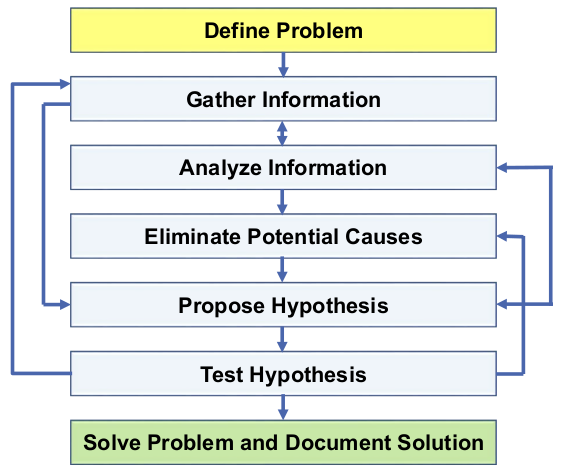
\includegraphics[width=0.7\linewidth]{img/img01}
	\end{center}
\end{frame}

\begin{frame}
	\frametitle{Troubleshooting Methods}
	\begin{center}
		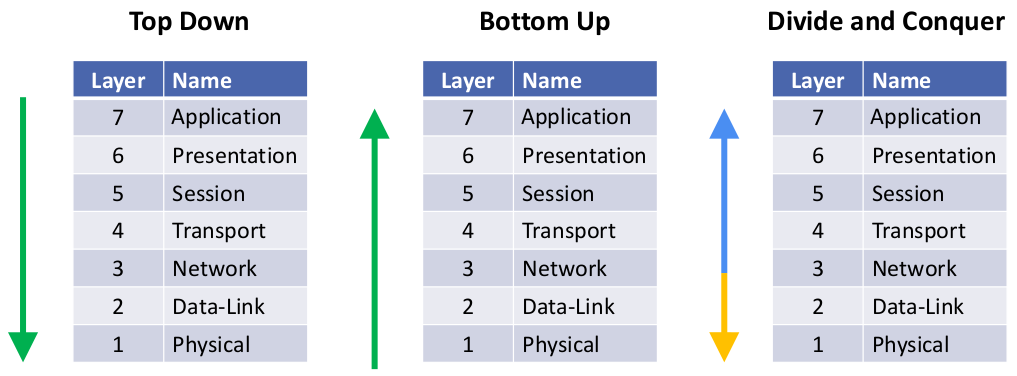
\includegraphics[width=\linewidth]{img/img02}
	\end{center}
\end{frame}

\begin{frame}{Troubleshooting Methods}
	\begin{itemize}
		\item Compare configurations
		\item Trace the path
		\item Swap out components
	\end{itemize}
\end{frame}

\begin{frame}{Connectivity Troubleshooting Methods}
	\begin{itemize}
		\item Ping
		\item Traceroute
		\item Telnet
	\end{itemize}
\end{frame}

\begin{frame}
	\begin{center}
		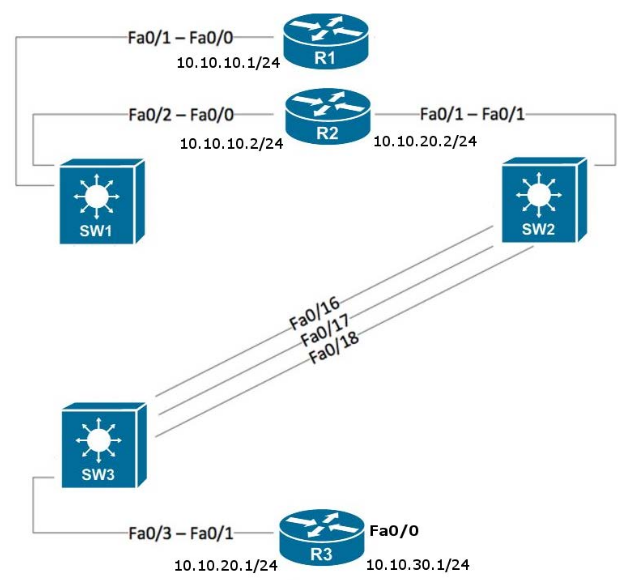
\includegraphics[height=0.8\textheight]{img/img03}
	\end{center}
\end{frame}

\end{document}
